\documentclass[border=10pt]{standalone}

\usepackage{tikz}
\usepackage{tikzsymbols}
\usetikzlibrary{calc,patterns,shapes.geometric}

\def\centerarc[#1](#2)(#3:#4:#5){\draw[#1] ($(#2)+({#5*cos(#3)},{#5*sin(#3)})$) arc (#3:#4:#5);}

\begin{document}
	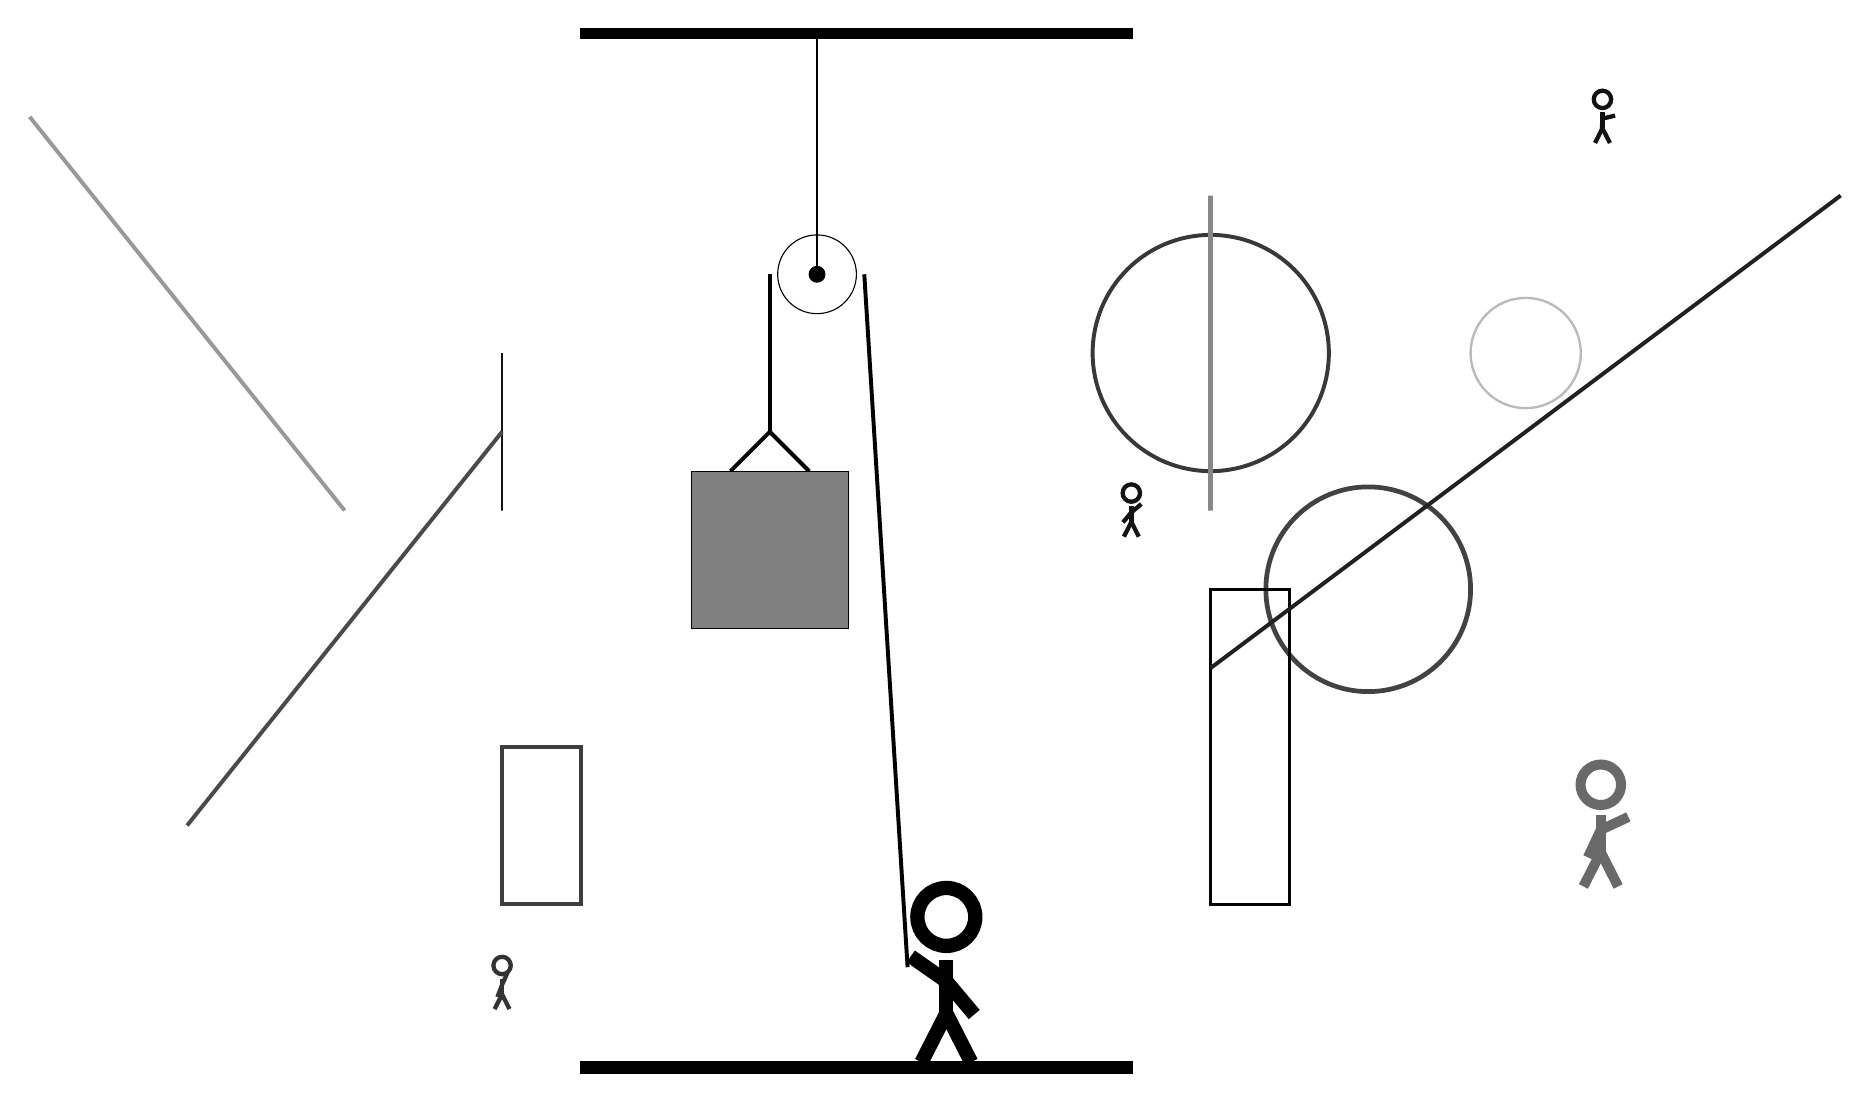
\begin{tikzpicture}
		%%%%% START %%%%%
		
		\draw[fill=black] (-2, 10) rectangle (5, 10.125);
		
		\draw (1, 7) circle (0.5);
		\draw[fill=black] (1, 7) circle (0.1);
		\draw (1, 10) -- (1, 7);
		
		\node[line width=0.7mm, color=black!93] at (11, 9) {\Strichmaxerl[3][87][14]};
		
		\draw [line width=0.5mm, color=black!78](6, 6) circle (1.5);
		\draw[line width=0.2mm, color=black!92] (-3, 6) rectangle (-3, 4);
		\draw [line width=0.6mm, color=black!74](8, 3) circle (1.3);
		\draw[line width=0.4mm, color=black!99] (6, -1) rectangle (7, 3);
		
		\node[line width=0.7mm, color=black!80] at (-3, -2) {\Strichmaxerl[3][69][66]};
		\draw[line width=0.5mm, color=black!87](6, 2) -- (14, 8);
		\node[line width=0.3mm, color=black!59] at (11, 0) {\Strichmaxerl[7][65][25]};
		\node[line width=0.7mm, color=black!92] at (5, 4) {\Strichmaxerl[3][50][40]};
		
		\draw[line width=0.5mm, color=black!40](-5, 4) -- (-9, 9);
		
		\draw[line width=0.5mm, color=black!76] (-2, -1) rectangle (-3, 1);
		
		\draw[line width=0.5mm, color=black!71](-3, 5) -- (-7, 0);
		\draw[line width=0.6mm, color=black!47] (6, 8) rectangle (6, 4);
		
		\draw [line width=0.3mm, color=black!27](10, 6) circle (0.7);
		
		\draw[line width=0.5mm] (-0.1, 4.5) -- (0.4, 5.0) -- (0.9, 4.5);
		\draw[fill=black!50] (-0.6, 4.5) rectangle (1.4, 2.5);
		
		\draw[line width=0.5mm] (0.4, 7) -- (0.4, 5.0);
		\centerarc[line width=0.5mm](1, 7)(0:180:0.6);
		\draw[line width=0.5mm](1.6, 7) -- (2.15, -1.8);
		
		\node at (2.6, -1.9) {\Strichmaxerl[10][-35][-50]};
		
		\draw[fill=black] (-2, -3) rectangle (5, -3.15);
		
		%%%%% END %%%%%
	\end{tikzpicture}
\end{document}